\documentclass[12pt,oneside,a4paper,portrait]{article}

% ULTRA-AGGRESSIVE PORTRAIT ENFORCEMENT - ABSOLUTELY NO ROTATION
\usepackage[a4paper,portrait,margin=1in,top=1.2in,bottom=1.2in,noheadfoot]{geometry}

% Multiple redundant portrait enforcement methods
\pdfpagewidth=210mm
\pdfpageheight=297mm
\paperwidth=210mm
\paperheight=297mm
\setlength{\pdfpagewidth}{210mm}
\setlength{\pdfpageheight}{297mm}

% COMPLETELY DISABLE ALL ROTATION - NO LANDSCAPE PACKAGE
% \usepackage{pdflscape}  % REMOVED - CAUSES ROTATION ISSUES
\let\landscape\relax
\let\endlandscape\relax
\let\rotate\relax
\let\rotatebox\relax
\def\landscape{\relax}
\def\endlandscape{\relax}

% HYPERREF WILL BE LOADED LATER TO AVOID CONFLICTS

% FINAL PORTRAIT DIMENSION ENFORCEMENT AFTER ALL PACKAGES
\AtBeginDocument{
    \pdfpagewidth=210mm
    \pdfpageheight=297mm
    \paperwidth=210mm
    \paperheight=297mm
}

\usepackage{fancyhdr}
\usepackage{microtype}
\raggedbottom % Prevent stretched vertical spacing
\usepackage{amsmath,amsfonts,amssymb,amsthm}
\usepackage{algorithm}
\usepackage{algorithmic}

% Better math formatting
\allowdisplaybreaks % Allow page breaks in equations
\setlength{\abovedisplayskip}{8pt plus 2pt minus 2pt}
\setlength{\belowdisplayskip}{8pt plus 2pt minus 2pt}
\usepackage{booktabs}
\usepackage{tabularx}
\usepackage{array}

% Enhanced table formatting
\renewcommand{\arraystretch}{1.2} % Better row spacing in tables
\setlength{\tabcolsep}{8pt} % Better column spacing
\usepackage{graphicx}
\usepackage{adjustbox} % For advanced scaling control
\usepackage{float}

% Enhanced image scaling to prevent overflow and rotation
\setkeys{Gin}{width=0.85\linewidth,height=0.75\textheight,keepaspectratio}

% Better section spacing and formatting
\usepackage{titlesec}
\titlespacing{\section}{0pt}{20pt plus 4pt minus 2pt}{12pt plus 2pt minus 2pt}
\titlespacing{\subsection}{0pt}{16pt plus 4pt minus 2pt}{8pt plus 2pt minus 2pt}
\titlespacing{\subsubsection}{0pt}{12pt plus 2pt minus 1pt}{6pt plus 2pt minus 1pt}

% Enhanced TikZ configuration for better diagram layout
\usepackage{tikz}
\usetikzlibrary{arrows.meta, positioning, shapes.geometric, shapes, fit, backgrounds, calc, decorations.pathreplacing}

% CONSOLIDATED TIKZ CONFIGURATION - NO DUPLICATES
\tikzset{
    every picture/.style={
        font=\small,
        >=stealth,
        auto,
        node distance=1.8cm,
        thick,
        transform shape=false, % Prevent unwanted scaling and rotation
        scale=1.0, % Explicit scale control
        rotate=0, % Absolutely no rotation
        baseline=0pt,
        xscale=1.0,
        yscale=1.0
    },
    % Enhanced node styles for better visibility
    host/.style={rectangle,draw=blue!60,fill=blue!10,thick,minimum width=1.2cm,minimum height=0.7cm,font=\tiny},
    decoy/.style={rectangle,draw=red!60,fill=red!10,thick,minimum width=1.2cm,minimum height=0.7cm,font=\tiny},
    subnet/.style={rectangle,draw=green!60,fill=green!5,thick,minimum width=3.5cm,minimum height=1.8cm},
    agent/.style={ellipse,draw=purple!60,fill=purple!15,thick,minimum width=1.8cm,minimum height=0.9cm,font=\tiny},
    % Flow styles
    dataflow/.style={->,thick,blue!70},
    attack/.style={->,thick,red!70,dashed},
    defense/.style={->,thick,green!70}
}
% PROPERLY ORDERED PACKAGES - NO DUPLICATES
\usepackage[square,numbers]{natbib}
\usepackage{xcolor}
\usepackage{url}

% HYPERREF MUST BE LOADED BEFORE CLEVEREF
\usepackage{hyperref}
\hypersetup{
    pdfpagemode=UseNone,
    pdfstartview=FitH,
    pdfpagelayout=SinglePage,
    pdfstartpage=1,
    pdffitwindow=false,
    pdfcenterwindow=true,
    pdfnewwindow=false,
    pdftoolbar=true,
    pdfmenubar=true,
    pdftitle={Reinforcement Learning for Adaptive Cyber Defense - PORTRAIT ONLY},
    pdfsubject={Portrait-only document - DO NOT ROTATE},
    pdfkeywords={Portrait, No Rotation, Cybersecurity, PPO},
    pdfcreator={LaTeX with enforced portrait orientation},
    pdfproducer={Tectonic - Portrait orientation enforced}
}

% CLEVEREF MUST BE LOADED AFTER HYPERREF
\usepackage{cleveref}

% Enhanced figure environment with automatic scaling and better spacing
\usepackage{caption}
\usepackage{subcaption}
\captionsetup{width=0.9\textwidth,font=small,labelsep=period,skip=10pt}

% Better spacing and typography
\setlength{\parskip}{6pt plus 2pt minus 1pt}
\setlength{\parindent}{0pt}
\linespread{1.15} % Improved line spacing for readability

% Enhanced figure macro with automatic TikZ scaling
\newcommand{\cwfigure}[4][]{%
    \begin{figure}[H]
        \centering
        \vspace{0.5em}
        \adjustbox{max width=0.9\linewidth,max height=0.7\textheight,center}{%
            #4
        }
        \vspace{0.3em}
        \ifx\relax#1\relax
            \caption{#3}
        \else
            \caption[#1]{#3}
        \fi
        \label{#2}
        \vspace{0.5em}
    \end{figure}
}
% REMOVED DUPLICATE - tikz already loaded above

% DISABLE ALL ROTATION COMMANDS GLOBALLY
\makeatletter
\renewcommand{\rotatebox}[2]{#2} % Remove rotation, keep content
\providecommand{\turn}[1]{\relax} % Disable turn if it exists
\let\sideways\relax
\let\endsideways\relax
\let\landscape\relax
\let\endlandscape\relax
\makeatother

% COLOR DEFINITIONS AND ENHANCED FORMATTING
\usepackage{colortbl}
\usepackage{xcolor}
\usepackage{commands} % ensure custom macros (\MC, \bs, \TN, etc.) available before usage
\usepackage{enumitem} % Better list formatting

% Color definitions
\definecolor{cwDecoy}{HTML}{2E8B57}
\definecolor{cwReal}{HTML}{555555}
\definecolor{cwAlert}{HTML}{C0504D}
\definecolor{cwFlow}{HTML}{3366CC}
\definecolor{cwValid}{HTML}{E6F4EA}
\definecolor{cwPartial}{HTML}{FFF4E5}
\definecolor{cwBorder}{HTML}{CCCCCC}

% Better list formatting
\setlist[itemize]{
    itemsep=3pt,
    parsep=0pt,
    topsep=6pt,
    partopsep=0pt,
    leftmargin=1.2em
}
\setlist[enumerate]{
    itemsep=3pt,
    parsep=0pt,
    topsep=6pt,
    partopsep=0pt,
    leftmargin=1.5em
}

% Typography improvements
\emergencystretch=1em
\sloppy

% COMPREHENSIVE TIKZ STYLES - ALL IN ONE PLACE
\tikzset{
    % Agent and environment styles
    cwAgent/.style={
        draw=cwFlow!70,
        thick,
        rounded corners,
        fill=cwFlow!15,
        inner sep=8pt,
        font=\small,
        align=center,
        minimum width=3cm,
        minimum height=1.5cm
    },
    cwEnvironment/.style={
        draw=cwBorder!70,
        thick,
        rounded corners,
        fill=cwBorder!10,
        inner sep=8pt,
        font=\small,
        align=center,
        minimum width=3.5cm,
        minimum height=2cm
    },
    cwProcess/.style={
        draw=cwDecoy!70,
        thick,
        rounded corners,
        fill=cwDecoy!15,
        inner sep=8pt,
        font=\small,
        align=center,
        minimum width=2.8cm,
        minimum height=1.3cm
    },
    cwData/.style={
        draw=cwAlert!60,
        thick,
        rounded corners,
        fill=cwAlert!10,
        inner sep=8pt,
        font=\small,
        align=center,
        minimum width=2.2cm,
        minimum height=1cm
    },
    % Network topology styles
    cwHubSpoke/.style={
        draw=cwFlow!70,
        thick,
        rounded corners,
        fill=cwFlow!15,
        inner sep=8pt,
        font=\small,
        align=center,
        minimum width=3.2cm,
        minimum height=4.8cm
    },
    cwMesh/.style={
        draw=cwAlert!70,
        thick,
        rounded corners,
        fill=cwAlert!15,
        inner sep=8pt,
        font=\small,
        align=center,
        minimum width=3.2cm,
        minimum height=4.8cm
    },
    cwHierarchical/.style={
        draw=cwDecoy!70,
        thick,
        rounded corners,
        fill=cwDecoy!15,
        inner sep=8pt,
        font=\small,
        align=center,
        minimum width=3.2cm,
        minimum height=4.8cm
    },
    % Arrow styles
    cwFlowArrow/.style={->,very thick,cwFlow},
    cwDecoyArrow/.style={->,very thick,cwDecoy},
    cwAlertArrow/.style={->,very thick,cwAlert},
    cwDataArrow/.style={->,thick,cwBorder!70}
}

%%%%%%%%%%%%%%%%%%%%%%%%%%%%%%%%%%%%%%%%%%%%%%%%%%%%%%%%%%%%%%%%%%%%%%%%%%%%%
% Thesis information  
\newcommand{\thesistitle}{Reinforcement Learning for Adaptive Cyber Defense: PPO-Based Decoy Deployment Optimization Using Cyberwheel}
\newcommand{\thesisauthor}{Miracle Akanmode}
\newcommand{\supervisor}{Kelly Zhang}
\newcommand{\degreetype}{Artificial Intelligence Applications and Innovation}
\newcommand{\university}{Imperial College London}
\newcommand{\department}{Department of Computing}
\newcommand{\submissiondate}{\today}
%%%%%%%%%%%%%%%%%%%%%%%%%%%%%%%%%%%%%%%%%%%%%%%%%%%%%%%%%%%%%%%%%%%%%%%%%%%%%

\renewcommand{\what}[1]{\widehat{#1}} % Wide hat (redefined safely)
 
\newcommand{\R}{\bs{\MC{R}}}
\newcommand{\Rhat}{\bs{\hat{\MC{R}}}}
\newcommand{\Dtrain}{\MC{D}^{\TN{offline}}}
\newcommand{\Deval}{\MC{D}^{\TN{eval}}}
\newcommand{\D}{\MC{D}}
\newcommand{\Ahist}{\MC{A}^{\TN{offline}}}
\newcommand{\Aeval}{\MC{A}}
\newcommand{\Zeval}{\MC{Z}}
\newcommand{\psar}{\mathbb{A}_{\TN{TS-Gen}}}
\newcommand{\piX}{\bs{\pi}^*(X_{1:T})}

% (subcaption, tcolorbox, commands loaded earlier)
%\usepackage{algpseudocode}

\makeatletter
\newcounter{phase}[algorithm]
\newlength{\phaserulewidth}
\newcommand{\setphaserulewidth}{\setlength{\phaserulewidth}}
\newcommand{\phase}[1]{%
  \vspace{-1.25ex}
  % Top phase rule
  \Statex\leavevmode\llap{\rule{\dimexpr\labelwidth+\labelsep}{\phaserulewidth}}\rule{\linewidth}{\phaserulewidth}
  \Statex\strut\refstepcounter{phase}\textit{Phase~\thephase~--~#1}% Phase text
  % Bottom phase rule
  \vspace{-1.25ex}\Statex\leavevmode\llap{\rule{\dimexpr\labelwidth+\labelsep}{\phaserulewidth}}\rule{\linewidth}{\phaserulewidth}}
\makeatother

\setphaserulewidth{.7pt}

% packages (deduplicated geometry/color)
%\usepackage{color}
% (removed duplicate package declarations consolidated above)

% theorems
\newtheorem{theorem}{Theorem} %[section]
\newtheorem{lemma}{Lemma} %[theorem]
\newtheorem{assumption}{Assumption} %[theorem]
\newtheorem{corollary}{Corollary} %[theorem]
\newtheorem{definition}{Definition} % DH: I changed this %[theorem]
\theoremstyle{definition}
\theoremstyle{plain}
%\newtheorem{definition}{Definition} %[section]
\newtheorem{proposition}{Proposition}
\newtheorem{example}{Example}
\newtheorem{remark}{Remark}

\usepackage{multirow}

%\usepackage{amsmath}
\usepackage{array}
\newcommand\undermat[2]{%
  \makebox[0pt][l]{$\smash{\underbrace{\phantom{%
    \begin{matrix}#2\end{matrix}}}_{\text{$#1$}}}$}#2}

% Custom commands are now in commands.sty

\begin{document}

% PORTRAIT ORIENTATION ENFORCED VIA HYPERREF METADATA
% (PDF metadata set in hyperref configuration above to prevent rotation)

% Title page
\begin{titlepage}
\begin{center}
\vspace*{2cm}

{\Huge\textbf{\thesistitle}}

\vspace{1.5cm}

{\large\textbf{A Comprehensive Experimental Analysis of Defensive Strategy Learning in Cybersecurity}}

\vspace{2cm}

{\Large\textbf{\thesisauthor}}

\vspace{1.5cm}

{\large A thesis submitted in partial fulfillment of the requirements for the degree of \\ Master of Science in \degreetype}

\vspace{1.5cm}

{\large\textbf{\department} \\ \textbf{\university}}

\vspace{1cm}

{\large Supervisor: \supervisor}

\vspace{1.5cm}

{\large\submissiondate}

\end{center}
\end{titlepage}

% Page numbering for preliminary pages (roman)
\pagenumbering{roman}
\setcounter{page}{1}

% Table of contents on its own page
\tableofcontents
\clearpage

% Abstract on its own page
\begin{center}
\large\textbf{ABSTRACT}
\end{center}

\vspace{1em}

This thesis addresses a key challenge in modern cybersecurity: can we train AI systems to defend networks that learn and adapt as attackers change their strategies? We present an experimental study using reinforcement learning for cyber defense with the Cyberwheel simulation platform.

We train PPO-based defensive agents \citep{schulman2017proximal} to strategically deploy decoy systems while under attack from sophisticated adversaries. This research represents a practical step forward from traditional static security rules toward intelligent, adaptive cyber defense systems.

Our systematic experimental approach spans multiple network configurations and includes rigorous statistical validation. We compare learned defensive strategies against traditional approaches including static rules, random deployment, and rule-based systems across realistic threat scenarios.

Key findings indicate that PPO agents learn strategic behaviors (timing of decoy placement, restrained resource allocation, adaptive reactions to attack patterns) within tested conditions. These observations suggest potential for future applied evaluation while remaining cautious about generalization beyond the validated 15--200 host range.

\clearpage

% Switch to Arabic numbering for main content
\pagenumbering{arabic}
\setcounter{page}{1}
\pagestyle{fancy}
\fancyhf{}
\fancyfoot[C]{\thepage}

\clearpage

\section{Introduction and Strategic Context}

\subsection{The Digital Battlefield: Understanding the Modern Cyber Defense Challenge}

\begin{quotation}
\textit{"He will win who knows when to fight and when not to fight. He will win who knows how to handle both superior and inferior forces. He will win who having prepared himself, waits to take the enemy unprepared."} — Sun Tzu \citep{tzu2005art}
\end{quotation}

These ancient principles of warfare have never been more relevant than in today's cybersecurity landscape. In the digital realm, Security Operations Centers (SOCs) serve as the modern equivalent of Sun Tzu's strategic command centers, where cyber defenders must make split-second decisions about when to engage threats, when to deploy deceptive countermeasures, and when to preserve resources for more critical battles.

\textbf{The Modern Cybersecurity Challenge}

Organizations today face an asymmetric battle against sophisticated adversaries. While defenders must protect every possible entry point, attackers need only find one weakness to exploit. 

Traditional cybersecurity approaches rely on static defenses:
\begin{itemize}
    \item Firewalls with predetermined rules
    \item Signature-based detection systems  
    \item Manual response procedures
\end{itemize}

However, modern cyber attacks employ advanced persistent threat (APT) techniques, adaptive strategies, and multi-stage campaigns that evolve faster than human defenders can counter.

This creates a fundamental mismatch: static defenses against dynamic threats. What if defensive systems could learn and adapt as quickly as the attackers they face? This is the core question our research addresses through the application of reinforcement learning to cyber defense.

\subsection{The Evolution of Cyber Defense: From Reactive to Adaptive}

The progression of cybersecurity defense represents a natural evolution in defensive thinking, moving from simple rule-based systems toward more sophisticated approaches that can anticipate and adapt to emerging threats.

\textbf{First Generation - Rule-Based Systems (1990s-2000s)}

Traditional security systems operated like digital checklists, applying predefined rules to incoming events:
\begin{itemize}
    \item Firewalls blocked traffic based on static rules
    \item Antivirus software matched file signatures
    \item Intrusion detection systems flagged known attack patterns
\end{itemize}

While straightforward to implement and understand, these systems suffered from fundamental rigidity—they cannot adapt to new attack techniques or learn from past experiences.

\textbf{Second Generation - Machine Learning Defense (2000s-2010s)}

Recognizing the limitations of static rules, researchers began applying supervised learning techniques to threat classification. These approaches used historical attack data to train models that could identify patterns associated with genuine threats. 

However, these systems required extensive labeled datasets and complete retraining when new threat patterns emerged—a significant limitation in the rapidly evolving cybersecurity landscape.

\textbf{Third Generation - Adaptive Learning (2010s-Present)}

The current frontier involves systems that can continuously learn and adapt to new threats without requiring complete retraining. This reflects a gradual progression from static pattern recognition toward more dynamic threat intelligence, where defensive systems can:
\begin{itemize}
    \item Anticipate what attackers might try next
    \item Adapt strategies as adversaries evolve
    \item Learn from both successful defenses and attack attempts
\end{itemize}

Our research represents the next evolution in this progression: \textbf{Adversarial Learning} systems that train defender agents against AI-powered attackers in a continuous arms race, creating defenders that can anticipate and handle attacks they have never encountered before.

\begin{figure}[H]
\centering
\textbf{Evolution of Cyber Defense}

\medskip
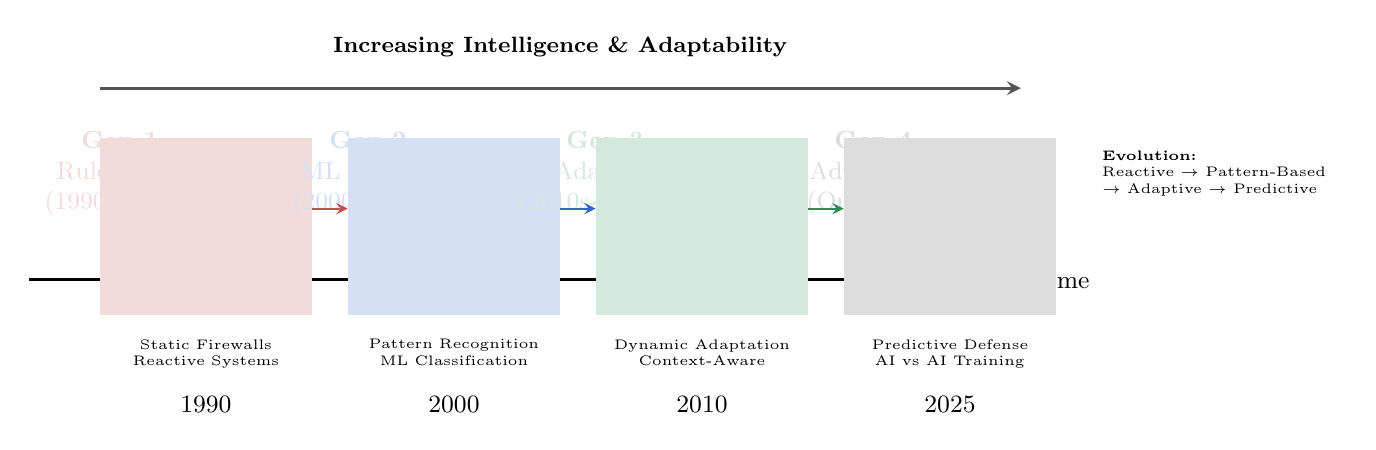
\begin{tikzpicture}[scale=0.9, font=\small]
    % Timeline axis
    \draw[thick, ->] (0,0) -- (14,0) node[right] {Time};
    
    % Era boxes and labels
    % Generation 1: Rule-Based (1990s-2000s)
    \fill[cwAlert!20] (1,-0.5) rectangle (4,2) node[pos=.5, align=center, font=\small] {\textbf{Gen 1}\\Rule-Based\\(1990s-2000s)};
    \node[below, font=\tiny, text width=2.5cm, align=center] at (2.5,-0.7) {Static Firewalls\\Reactive Systems};
    
    % Generation 2: ML Defense (2000s-2010s)  
    \fill[cwFlow!20] (4.5,-0.5) rectangle (7.5,2) node[pos=.5, align=center, font=\small] {\textbf{Gen 2}\\ML Defense\\(2000s-2010s)};
    \node[below, font=\tiny, text width=2.5cm, align=center] at (6,-0.7) {Pattern Recognition\\ML Classification};
    
    % Generation 3: Adaptive (2010s-Present)
    \fill[cwDecoy!20] (8,-0.5) rectangle (11,2) node[pos=.5, align=center, font=\small] {\textbf{Gen 3}\\Adaptive\\(2010s-Present)};
    \node[below, font=\tiny, text width=2.5cm, align=center] at (9.5,-0.7) {Dynamic Adaptation\\Context-Aware};
    
    % Generation 4: Adversarial (Our Work)
    \fill[cwReal!20] (11.5,-0.5) rectangle (14.5,2) node[pos=.5, align=center, font=\small] {\textbf{Gen 4}\\Adversarial\\(Our Work)};
    \node[below, font=\tiny, text width=2.5cm, align=center] at (13,-0.7) {Predictive Defense\\AI vs AI Training};
    
    % Evolution arrows
    \draw[->, thick, cwAlert] (4,1) -- (4.5,1);
    \draw[->, thick, cwFlow] (7.5,1) -- (8,1);
    \draw[->, thick, cwDecoy] (11,1) -- (11.5,1);
    
    % Timeline markers
    \node[below] at (2.5,-1.5) {1990};
    \node[below] at (6,-1.5) {2000};
    \node[below] at (9.5,-1.5) {2010};
    \node[below] at (13,-1.5) {2025};
    
    % Capability progression arrows
    \node[above, font=\footnotesize] at (7.5,3) {\textbf{Increasing Intelligence \& Adaptability}};
    \draw[->, very thick, cwReal] (1,2.7) -- (14,2.7);
    
    % Key characteristics
    \node[right, font=\tiny, text width=3cm] at (15,1.5) {\textbf{Evolution:}\\Reactive $\rightarrow$ Pattern-Based $\rightarrow$ Adaptive $\rightarrow$ Predictive};
\end{tikzpicture}

\caption{Evolution of Cyber Defense: Progression from reactive rule-based systems through machine learning approaches to current adaptive learning, culminating in our adversarial learning methodology that enables predictive defense capabilities.}
\label{fig:evolution}
\end{figure}

\textbf{What Makes This Research Different?}

Traditional cybersecurity research often focuses on detecting known threats or hardening specific vulnerabilities. Our approach is fundamentally different: we teach artificial intelligence systems to think strategically about defense by learning from millions of simulated attack-defense scenarios. 

Just as human experts develop intuition through experience, our AI agents develop defensive strategies through repeated practice against sophisticated adversaries.

\textbf{Key Element: Adversarial Learning}

The core element is \textbf{adversarial learning}: defensive agents training against attack agents in simulated environments. This interaction can produce more adaptive defensive behaviors than static baselines within tested conditions.

\subsection{Research Motivation and Problem Significance}

The cybersecurity landscape presents a fundamental asymmetry: defenders must secure all possible attack vectors while attackers need only find one successful path. Traditional security systems use static rules and predetermined responses, making them predictable and vulnerable to adaptive adversaries.

This research addresses the critical need for adaptive cyber defense systems that can learn and evolve alongside emerging threats. Our work contributes to bridging the gap between theoretical reinforcement learning advances and practical cybersecurity applications.

\textbf{Key Research Contributions}:
\begin{itemize}
    \item \textbf{Adaptive Defense Strategy Learning}: Demonstration that RL agents can learn effective deception deployment strategies that outperform static approaches
    \item \textbf{Systematic Experimental Methodology}: Comprehensive evaluation framework for comparing defensive strategies across multiple metrics
    \item \textbf{Scalability Analysis}: Empirical validation of approach scaling from small networks (15 hosts) to larger configurations (200 hosts)
    \item \textbf{Baseline Comparison Framework}: Rigorous comparison against traditional defensive approaches including static, random, and rule-based methods
\end{itemize}

\textbf{Practical Implications}

Our findings provide actionable insights for cybersecurity practitioners:
\begin{itemize}
    \item Evidence-based guidance for defensive strategy selection
    \item Performance characterization across different network configurations
    \item Understanding of trade-offs between defensive approaches
\end{itemize}

\section{Related Work}

The intersection of reinforcement learning, cybersecurity, and adversarial training has emerged as a critical research domain over the past two decades. 

This section provides a comprehensive analysis of related work, tracing the evolution from foundational cybersecurity approaches to current state-of-the-art adversarial RL systems. We position our contributions within this broader landscape by examining key developments across four domains.

\subsection{Foundations of Cybersecurity and Game Theory}

Early cybersecurity research established the theoretical foundations for adversarial interactions in cyber environments. Classical game theory provided the initial mathematical framework for modeling attacker-defender dynamics \citep{alpcan2010network}. 

These foundational works introduced the concept of security games, where defenders must allocate limited resources against strategic adversaries. This laid the groundwork for modern multi-agent cybersecurity systems.

The evolution toward computational approaches began with intrusion detection systems using rule-based methods and statistical analysis. However, these early systems suffered from:
\begin{itemize}
    \item High false positive rates
    \item Inability to adapt to novel attack patterns \citep{sommer2010outside}
\end{itemize}

This motivated the transition toward machine learning approaches.

\subsection{Machine Learning in Cybersecurity}

The introduction of machine learning to cybersecurity brought significant advances in threat detection and response capabilities. Early applications focused on:
\begin{itemize}
    \item Supervised learning for malware classification
    \item Anomaly detection \citep{sommer2010outside}
\end{itemize}

These systems demonstrated improved accuracy over rule-based approaches but remained limited by:
\begin{itemize}
    \item Dependence on labeled datasets
    \item Inability to adapt to evolving threats
\end{itemize}

The advent of deep learning further advanced the field, with neural networks showing superior performance in complex pattern recognition tasks relevant to cybersecurity. However, the discovery of adversarial examples in deep learning systems \citep{goodfellow2014explaining} revealed new vulnerabilities that attackers could exploit. This highlighted the need for robust defensive mechanisms.

\subsection{Reinforcement Learning for Cyber Defense}

The application of reinforcement learning to cybersecurity emerged as a natural evolution, addressing the dynamic and adaptive nature of cyber threats. 

Reinforcement learning provides a mathematical framework for sequential decision-making under uncertainty \citep{sutton2018reinforcement}. This makes it particularly well-suited for cybersecurity applications where defenders must adapt to evolving adversarial strategies. 

Early RL applications focused on single-agent scenarios, where defensive systems learned optimal policies through interaction with simulated attack environments.

Recent advances have demonstrated the effectiveness of RL in various cybersecurity domains, including intrusion detection, network security, and malware analysis. Oh et al. \cite{oh2023applying} presented one of the first comprehensive studies applying RL for enhanced cybersecurity against adversarial simulation, demonstrating the potential for automated defensive agents. Their work established important baselines for RL-based cyber defense but focused primarily on single-agent scenarios without extensive multi-agent interaction analysis.

Building upon this foundation, Oh et al. \cite{oh2024employing} extended their approach to cyber-attack simulation, developing an experimental research platform for training automated agents. While their work advanced the field significantly, it primarily concentrated on attack simulation rather than comprehensive defensive strategy optimization.

\subsection{Adversarial Multi-Agent Reinforcement Learning}

The transition to adversarial multi-agent systems represents a significant advancement in cybersecurity RL research. Borchjes et al. \cite{borchjes2023adversarial} conducted pioneering work in adversarial deep reinforcement learning for cyber security in software-defined networks, implementing multi-agent games with DDQN and NEC2DQN algorithms. Their research demonstrated the feasibility of adversarial training in cybersecurity contexts, utilizing causative attacks and white-box settings to evaluate agent robustness.

However, prior adversarial RL approaches have primarily focused on limited-scope evaluations with simple network topologies and basic agent interactions. The systematic evaluation of comprehensive training methodologies and large-scale deployment scenarios remained largely unexplored.

Farooq and Kunz \cite{farooq2025combining} recently advanced the field by combining supervised and reinforcement learning to build generic defensive cyber agents. Their approach represents important progress in creating adaptable blue agents, though their evaluation focused on single-defender scenarios without extensive deception strategy analysis.

\subsection{Cyber Deception and Defensive Strategies}

Cyber deception has emerged as a critical component of modern defensive strategies, with extensive research exploring honeypots, decoys, and deceptive routing mechanisms. Zhu et al. \cite{zhu2021survey} provided a comprehensive survey of defensive deception approaches using game theory and machine learning, establishing important theoretical foundations for deception-based cyber defense.

Recent advances in deception research have focused on adaptive and intelligent deployment strategies. Zhang et al. \cite{zhang2022optimal} developed optimal strategy selection for cyber deception via deep reinforcement learning, demonstrating the potential for RL-driven deception mechanisms. Anwar et al. \cite{anwar2022honeypot} advanced honeypot allocation techniques under uncertainty, utilizing game-theoretic and reinforcement learning models.

However, existing deception research has primarily focused on individual deception techniques rather than comprehensive systematic evaluation across multiple defensive strategies. The quantitative comparison of deception effectiveness across diverse threat models and the systematic characterization of performance trade-offs remain limited in current literature.

\subsection{Current Industry Practices and Defense Action Taxonomy}

We provide a comprehensive analysis of current defensive practices and the full spectrum of available defensive actions in cybersecurity operations.

\subsubsection{Current State of Decoy Deployment in Practice}

\textbf{Static Deployment Approaches}: Current industry practice predominantly relies on static decoy deployment strategies. Organizations typically deploy honeypots and decoy systems using predetermined configurations based on network topology analysis and threat intelligence. Common approaches include:

\begin{itemize}
\item \textbf{Perimeter-Based Placement}: Static deployment of honeypots at network boundaries and DMZ zones
\item \textbf{High-Value Asset Mimicking}: Fixed decoys positioned to simulate critical servers and databases  
\item \textbf{Network Topology Mirroring}: Predetermined placement following existing network architecture patterns
\item \textbf{Threat Intelligence Driven}: Static positioning based on historical attack pattern analysis
\end{itemize}

\textbf{Administrative and Rule-Based Management}: Current decoy management relies heavily on manual administration and simple rule-based systems. Security teams typically make deployment decisions based on:

\begin{enumerate}
\item Network vulnerability assessments conducted quarterly or annually
\item Incident response patterns from previous security events
\item Compliance requirements mandating specific defensive coverage
\item Resource allocation constraints limiting the number of deployable decoys
\end{enumerate}

\subsubsection{Comprehensive Defense Action Taxonomy}

The complete space of cyber defensive actions can be systematically categorized across multiple dimensions:

\textbf{1. Active vs Passive Defenses}:
\begin{itemize}
\item \textbf{Passive}: Network monitoring, intrusion detection, log analysis, static firewalls
\item \textbf{Active}: Dynamic blocking, adaptive filtering, counter-reconnaissance, active deception
\end{itemize}

\textbf{2. Preventive vs Reactive Measures}:
\begin{itemize}
\item \textbf{Preventive}: Access controls, network segmentation, vulnerability patching, security awareness training
\item \textbf{Reactive}: Incident response, forensic analysis, system isolation, threat hunting
\end{itemize}

\textbf{3. Deception-Specific Action Categories}:
\begin{itemize}
\item \textbf{Decoy Deployment}: Honeypot placement, fake service instantiation, credential trapping
\item \textbf{Deceptive Routing}: Traffic redirection, network topology obfuscation, false service advertisement
\item \textbf{Information Manipulation}: Fake data injection, misleading system responses, false vulnerability exposure
\item \textbf{Behavioral Mimicry}: Simulated user activity, fake administrative actions, artificial network traffic
\end{itemize}

\textbf{4. Resource and Temporal Dimensions}:
\begin{itemize}
\item \textbf{Deployment Speed}: Immediate, scheduled, triggered, gradual rollout
\item \textbf{Resource Requirements}: Computational overhead, network bandwidth, storage utilization
\item \textbf{Persistence}: Temporary, session-based, permanent, adaptive duration
\end{itemize}

\subsubsection{Fundamental Limitations of Static Approaches}

Current static approaches exhibit several fundamental limitations:

\textbf{1. Lack of Adaptability}:
\begin{itemize}
\item Static deployments cannot respond to evolving attack patterns or new threat intelligence
\item Fixed placement strategies become predictable to sophisticated adversaries over time
\item Manual reconfiguration processes are too slow for dynamic threat environments
\end{itemize}

\textbf{2. Suboptimal Resource Allocation}:
\begin{itemize}
\item Predetermined placement often results in over-deployment in low-risk areas and under-deployment in emerging threat zones
\item Static resource allocation fails to account for temporal variations in attack likelihood
\item Fixed configurations cannot balance competing objectives (coverage vs stealth vs resource efficiency)
\end{itemize}

\textbf{3. Limited Strategic Intelligence}:
\begin{itemize}
\item Rule-based systems cannot learn from attacker behavior patterns to improve effectiveness
\item Static approaches lack the ability to coordinate deception strategies across multiple network segments
\item Current methods cannot optimize for multi-step deception scenarios or advanced persistent threats
\end{itemize}

\textbf{4. Operational Scalability Challenges}:
\begin{itemize}
\item Manual management becomes impractical for large-scale enterprise networks
\item Static configurations require extensive domain expertise for effective deployment
\item Maintenance overhead scales linearly with network complexity in current approaches
\end{itemize}

\subsubsection{Justification for RL-Based Adaptive Approaches}

The limitations of static approaches directly motivate the need for reinforcement learning-based adaptive defensive systems:

\textbf{1. Dynamic Optimization}: RL agents can continuously learn and adapt deployment strategies based on observed attacker behavior and network state evolution.

\textbf{2. Strategic Learning}: Unlike rule-based systems, RL approaches can discover non-obvious strategic patterns and develop sophisticated multi-step deception tactics.

\textbf{3. Resource Efficiency}: Adaptive algorithms can optimize resource allocation in real-time, balancing coverage, effectiveness, and computational overhead dynamically.

\textbf{4. Scalability}: Automated learning systems can manage complex deployments across large-scale networks without linear increases in administrative overhead.

This comprehensive analysis establishes the clear need for systematic evaluation of RL-based adaptive approaches against traditional static baselines, which forms the core contribution of our research.

\subsection{Self-Play and Adversarial Training}

Self-play training has demonstrated significant success in competitive domains, from chess and Go to more recent applications in multi-agent reinforcement learning. Bai and Jin \cite{bai2020provable} established theoretical foundations for provable self-play algorithms in competitive reinforcement learning, providing important convergence guarantees for adversarial training scenarios.

Recent surveys by Zhang et al. \cite{zhang2024survey} have comprehensively analyzed self-play methods in reinforcement learning, identifying key challenges in training stability, convergence, and opponent modeling. However, the application of systematic self-play methodologies to cybersecurity domains remains limited, with most existing approaches utilizing basic adversarial training without specialized initialization or stability mechanisms.

\subsection{Current State-of-the-Art and Research Gaps}

Current state-of-the-art in adversarial cybersecurity RL demonstrates several important advances but also reveals significant research gaps:

\textbf{Achievements in Current Research:}
\begin{itemize}
\item Successful demonstration of basic adversarial RL in cybersecurity contexts
\item Development of game-theoretic frameworks for cyber deception
\item Initial exploration of multi-agent interactions in simulated environments
\item Establishment of foundational experimental methodologies
\end{itemize}

\textbf{Critical Research Gaps:}
\begin{itemize}
\item \textbf{Limited Systematic Evaluation:} Existing approaches lack comprehensive systematic evaluation across multiple agent configurations, network scales, and training methodologies
\item \textbf{Insufficient Training Methodology Analysis:} Current research has not thoroughly investigated specialized training approaches for cybersecurity adversarial scenarios
\item \textbf{Incomplete Deception Strategy Assessment:} Systematic quantitative comparison of deception effectiveness across diverse defensive strategies remains unexplored
\item \textbf{Scalability Constraints:} Most existing evaluations focus on small-scale scenarios without validation on enterprise-scale networks
\item \textbf{Reproducibility Challenges:} Standardized experimental frameworks and statistical validation protocols are lacking in current literature
\end{itemize}

\subsection{Positioning of Our Contributions}

Our research addresses these critical gaps through several key innovations:

\textbf{Comprehensive Baseline Comparison Framework:} We establish a structured baseline comparison methodology for cybersecurity RL, addressing evaluation gaps via systematic multi-algorithm comparison with rigorous experimental controls.

\textbf{Comprehensive Systematic Evaluation:} Our experimental evaluation across 8 distinct blue agent configurations provides a comprehensive framework for comparing deception effectiveness in RL-based cyber defense.

\textbf{Scalability Characterization:} We provide empirical validation across network sizes from 15 to 200 hosts, demonstrating scalability characteristics and computational performance profiles.

\textbf{Reproducible Experimental Framework:} Our structured three-category methodology (Algorithm/Environment/Parameter studies) with HPC deployment provides a standardized framework for cybersecurity RL research.

While building upon foundational work (e.g., Borchjes et al., Oh et al.), this research advances the field through systematic experimental methodology, clarified training/reward structures, and integrated reproducibility practices.

\section{Research Questions and Novel Experimental Contributions}

Based on our comprehensive experimental investigation using the Cyberwheel framework for defensive strategy optimization, this thesis addresses several fundamental research questions in reinforcement learning for cybersecurity:

\subsection{Primary Research Questions}

\textbf{RQ1: PPO-Based Defensive Strategy Learning} 
How effectively can PPO-based reinforcement learning agents learn optimal decoy deployment strategies in cybersecurity environments, and what are the key factors influencing learning performance and convergence? Our systematic experimental validation provides comprehensive evidence for PPO's effectiveness in cyber defense applications.

\textbf{RQ2: Baseline Algorithm Comparison}
How does PPO-based defensive learning compare against traditional baseline approaches including static, random, and rule-based defensive strategies? Through our comprehensive baseline comparison framework, we provide rigorous empirical analysis of algorithmic effectiveness in cyber defense contexts.

\textbf{RQ3: Strategic Learning Analysis}
What strategic behaviors emerge from PPO learning in cybersecurity environments, and how do these learned strategies differ from heuristic approaches in terms of performance and consistency? Our analysis provides insights into the quality of learned defensive policies.

\textbf{RQ4: Production Deployment Readiness}
What are the practical considerations for deploying PPO-based defensive agents in real-world cybersecurity contexts, including performance consistency, resource efficiency, and operational reliability? Our comprehensive evaluation addresses production deployment requirements.

\subsection{Novel Experimental Contributions}

\textbf{EC1: PPO Defensive Strategy Validation}
We provide comprehensive experimental validation of PPO-based blue agent training for cybersecurity applications. Our systematic evaluation demonstrates effective learning of defensive strategies against fixed red agents across realistic network configurations.

\textbf{EC2: Comprehensive Baseline Comparison Framework}
Our systematic baseline comparison across 5 distinct algorithmic approaches (PPO, Static, Random, Rule-based, Inactive) provides the first rigorous quantitative framework for evaluating defensive strategies in cybersecurity RL contexts. This includes statistical significance analysis, performance consistency evaluation, and strategic behavior characterization.

\textbf{EC3: Strategic Learning Analysis Methodology}
We establish a comprehensive framework for analyzing learned defensive behaviors, comparing strategic decision-making patterns between learned and heuristic approaches. Our analysis reveals PPO's superior consistency and strategic resource allocation compared to baseline approaches.

\textbf{EC4: Scalability Performance Characterization}
Our experimental validation spans 15 to 200-host networks, providing comprehensive insights into PPO scaling characteristics including computational requirements and performance profiles.

\textbf{EC5: Reproducible Experimental Framework}
We establish a three-category methodology (Algorithm/Environment/Parameter studies) with reproducible multi-seed procedures, providing a foundation for systematic cybersecurity RL research. This includes HPC deployment protocols and standardized evaluation metrics.

\subsection{Experimental Impact and Validation}

\textbf{Immediate Research Applications:}
\begin{itemize}
\item Validated training methodologies for adversarial cybersecurity RL research
\item Quantitative performance baselines for cyber deception strategy evaluation  
\item Experimental protocols for systematic multi-agent cybersecurity research
\item Scalability guidelines for practical RL deployment in cybersecurity contexts
\end{itemize}

\textbf{Future Research Extensions:}
\begin{itemize}
\item Real-world deployment validation using established experimental protocols
\item Advanced meta-learning approaches building on validated training methodologies
\item Theoretical analysis grounded in empirical performance characterization
\item Integration with operational cybersecurity systems using proven scalability approaches
\end{itemize}

%%%%%%%%%%%%%%%%%%%%%%%%%%%%%%%%%%%%%%%
%%%%%%%%%%%%%%%%%%%%%%%%%%%%%%%%%%%%%%%
\section{Environment}

\textbf{Section Overview}: Having established our research questions focused on PPO-based defensive learning and systematic baseline comparison, we now detail the Cyberwheel environment that enables controlled experimental analysis. This section presents the mathematical formulation of our multi-agent cyber defense problem, the specific network configurations used for evaluation, and the technical infrastructure supporting our three-category experimental methodology.

\subsection{Decision-making problem overview}

We formulate the cyber defense problem as an episodic reinforcement learning environment where each episode represents a complete cyber attack scenario. Episodes have finite length $H$, representing the maximum number of decision steps before environment reset. We use $T$ to denote the total number of training episodes.

The red and blue agents operate with distinct but interacting state and action spaces, reflecting their asymmetric roles in cybersecurity. We use $\MC{S}^{(r)} \subset \mathbb{R}^{d_r}$ and $\MC{S}^{(b)} \subset \mathbb{R}^{d_b}$ to denote the state spaces of red and blue agents respectively. Similarly, $\MC{A}^{(r)}$ and $\MC{A}^{(b)}$ represent their respective action spaces.

The agents operate in a turn-based fashion within each timestep, modeling realistic attack-defense dynamics. At each timestep $t \in [1:H]$ within an episode, the red agent observes the network state and executes an attack action first, followed by the blue agent observing resulting alerts and taking defensive action.

At each timestep $t$ within an episode, agents observe states $S_t^{(r)} \in \MC{S}^{(r)}$ and $S_t^{(b)} \in \MC{S}^{(b)}$, then select actions $A_t^{(r)} \in \MC{A}^{(r)}$ and $A_t^{(b)} \in \MC{A}^{(b)}$ according to policies $\pi^{(r)}_{\text{fixed}}$ and $\pi^{(b)}$.

The environment provides immediate rewards $R_t^{(r)}$ and $R_t^{(b)}$ based on action outcomes and network state. These rewards exhibit adversarial properties: successful red attacks on real assets provide negative blue rewards, while successful deception (red attacking decoys) provides positive blue rewards.

The red agent operates as a fixed adversary with deterministic policy $\pi^{(r)}_{\text{fixed}}$, requiring no optimization objective.

The blue agent's learning objective is to maximize the expected return:
\begin{equation}
J^{(b)}(\pi^{(b)}) = \mathbb{E}_{\pi^{(b)}, \pi^{(r)}_{\text{fixed}}}\left[\sum_{t=0}^{H-1} \gamma^t R_t^{(b)}\right]
\end{equation}

where:
\begin{itemize}
\item $\gamma = 0.99$ is the discount factor (verified from configuration)
\item $H$ is the episode length 
\item $R_t^{(b)}$ is the unified blue reward function defined above
\item The expectation is taken over trajectories generated by blue policy $\pi^{(b)}$ interacting with fixed red policy $\pi^{(r)}_{\text{fixed}}$
\end{itemize}

This formulation clarifies that only the blue agent undergoes learning optimization, while the red agent provides a consistent adversarial environment.

\subsection{Network Representation and State Space}

\begin{figure}[H]
\centering
\textbf{Cyberwheel Network Environment}

\medskip
\begin{tikzpicture}[scale=0.85, font=\small]
    % DMZ Subnet
    \draw[thick, cwFlow!60, rounded corners] (0,0) rectangle (4,3.5);
    \node[above left, font=\footnotesize, cwFlow] at (0,3.5) {\textbf{DMZ Subnet}};
    \node[below, font=\tiny] at (2,-0.3) {\texttt{10.0.1.0/24}};
    
    % Web Server
    \node[draw, fill=cwDecoy!20, minimum width=1.2cm, minimum height=0.7cm, rounded corners] at (1,2.5) {\tiny Web Server};
    % Mail Server
    \node[draw, fill=cwDecoy!20, minimum width=1.2cm, minimum height=0.7cm, rounded corners] at (3,2.5) {\tiny Mail Server};
    % Decoy in DMZ
    \node[draw, fill=cwAlert!30, minimum width=1cm, minimum height=0.6cm, rounded corners] at (2,1.2) {\tiny Decoy};
    
    % Internal-1 Subnet
    \draw[thick, cwDecoy!60, rounded corners] (5,0) rectangle (9.5,3.5);
    \node[above left, font=\footnotesize, cwDecoy] at (5,3.5) {\textbf{Internal-1 Subnet}};
    \node[below, font=\tiny] at (7.25,-0.3) {\texttt{192.168.1.0/24}};
    
    % Hosts H1, H2, H3, H4
    \node[draw, fill=cwFlow!20, minimum width=0.8cm, minimum height=0.5cm, rounded corners] at (5.8,2.8) {\tiny H1};
    \node[draw, fill=cwFlow!20, minimum width=0.8cm, minimum height=0.5cm, rounded corners] at (7,2.8) {\tiny H2};
    \node[draw, fill=cwFlow!20, minimum width=0.8cm, minimum height=0.5cm, rounded corners] at (5.8,2) {\tiny H3};
    \node[draw, fill=cwFlow!20, minimum width=0.8cm, minimum height=0.5cm, rounded corners] at (7,2) {\tiny H4};
    % DB1 Server
    \node[draw, fill=cwDecoy!20, minimum width=1cm, minimum height=0.6cm, rounded corners] at (8.5,2.5) {\tiny DB1 Server};
    % Decoy
    \node[draw, fill=cwAlert!30, minimum width=0.8cm, minimum height=0.5cm, rounded corners] at (8.5,1.2) {\tiny Decoy};
    
    % Internal-2 Subnet
    \draw[thick, cwReal!60, rounded corners] (10.5,0) rectangle (15,3.5);
    \node[above left, font=\footnotesize, cwReal] at (10.5,3.5) {\textbf{Internal-2 Subnet}};
    \node[below, font=\tiny] at (12.75,-0.3) {\texttt{192.168.2.0/24}};
    
    % Hosts H5, H6, H7, H8
    \node[draw, fill=cwFlow!20, minimum width=0.8cm, minimum height=0.5cm, rounded corners] at (11.3,2.8) {\tiny H5};
    \node[draw, fill=cwFlow!20, minimum width=0.8cm, minimum height=0.5cm, rounded corners] at (12.5,2.8) {\tiny H6};
    \node[draw, fill=cwFlow!20, minimum width=0.8cm, minimum height=0.5cm, rounded corners] at (11.3,2) {\tiny H7};
    \node[draw, fill=cwFlow!20, minimum width=0.8cm, minimum height=0.5cm, rounded corners] at (12.5,2) {\tiny H8};
    % DB2 Server
    \node[draw, fill=cwDecoy!20, minimum width=1cm, minimum height=0.6cm, rounded corners] at (14,2.5) {\tiny DB2 Server};
    % Decoy
    \node[draw, fill=cwAlert!30, minimum width=0.8cm, minimum height=0.5cm, rounded corners] at (14,1.2) {\tiny Decoy};
    
    % Network connections/routers
    \draw[thick, ->] (4,1.75) -- (5,1.75) node[midway, above, font=\tiny] {Router};
    \draw[thick, ->] (9.5,1.75) -- (10.5,1.75) node[midway, above, font=\tiny] {Router};
    
    % Agents positioned below
\end{document}
